\section{Implementation and Deployment}

Our implementation of \system{} includes relays, an oracle, and 
a client. \system{} is open source and written in Python; the oracle is written in just 
175 lines of code and the relay is written in just under 200 lines of code.  \system{} is currently deployed globally, and
any user may use it today.  We have released an anonymized source code repository,
complete with usage instructions~\cite{ran_system}.

We assume that users and machines are trustworthy, and therefore the system runs 
securely.  This implementation of \system{} allows a client to avoid a single country 
at a time; attacks on \system{}, such as Denial of Service attacks and targetted 
surveillance of the relays, are outside the scope of the paper.

\paragraph{Relays}  The current deployment has ten relays, one in each
of the following
countries: Brazil,  Germany, Singapore, Japan, Australia, France, United
States, United Kingdom, Netherlands, and Canada; Figure~\ref{fig:relay_locations}
shows these relay locations, along with their corresponding ASes. These relays operate
as Ubuntu Virtual Private Servers (VPSes) with Squid as the proxy
server and the \system{} Relay software.

\begin{figure}[t!]
\centering
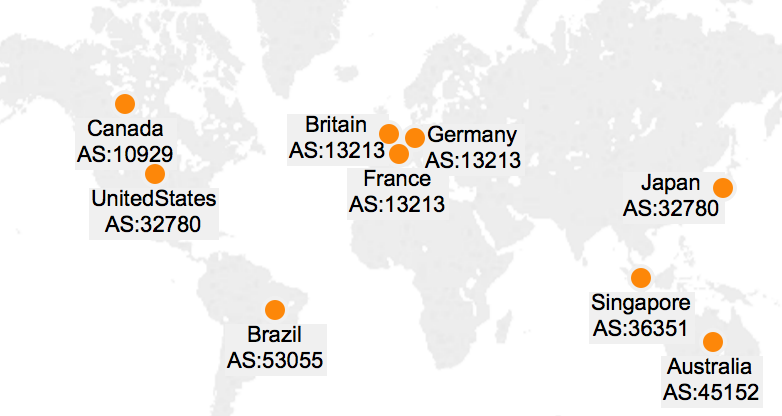
\includegraphics[width=.4\textwidth]{relay_map}
\caption{The locations and ASNs for \system{} relays.}
\label{fig:relay_locations}
\end{figure}

\paragraph{Oracle}  The oracle software runs on a Fujitsu RX200 S8 server with dual, 
eight-core 2.8~GHz Intel Xeon E5 2680 v2 processors with 256GB RAM running 
RedHat Linux. 

\paragraph{Client} To evaluate the \system{} deployment, we set up a client 
machine in the Netherlands, which simply accesses web content and uses the PAC 
file generated by the oracle. 

\subsection{Other Considerations}
%Adding relays to \system{} is 
%straightforward. Additionally, \system{} is resilient to failures of system components.

\paragraph{Adding relays and oracles} To add a relay, the system
operator must set up a machine as a proxy server, install the relay
software, and update the oracle's list of relays.  From that point
onward, paths will be computed to and from the new relay, and clients
will begin using the new proxy.  Adding an oracle requires installing
the oracle software on a different machine, and specifying the client
locations handled by that oracle (\eg, one oracle handles clients in
North America and Europe, and another handles clients elsewhere).
Both oracles will publish the PAC files to the same server, which
causes no changes for the client.

\paragraph{Failed relays and oracles} Unresponsive relays are handled
by the PAC file.  The PAC file allows the oracle to specify multiple
proxies in a sequential order, such that if the the first proxy fails,
then the client uses the second proxy (and so on).  This feature can
be used to specify all of the relays that have a path to the domain.
%And future work can include relay replicas that can be used in the
%case that a relay crashes.  
Among other mechanisms, we can detect a failed oracle by determining
that its PAC file is older than one hour.  Detecting a failed oracle
could trigger a backup oracle to re-compute the PAC files
periodically.  Because oracles are stateless, failover is
straightforward.  Without backup oracles, clients can still use the
system when the oracle fails.  The clients will simply be using stale
paths, which are likely (but not guaranteed) to be functional, since
country-level paths change infrequently.

